%%%%%%%%%%%%%%%%%%%%%%%%%%%%%%%%%%%%%%%%%%  不使用 authblk 包制作标题  %%%%%%%%%%%%%%%%%%%%%%%%%%%%%%%%%%%%%%%%%%%%%%
%-------------------------------PPT Title-------------------------------------
\title{\rm{Python}简介}
%-----------------------------------------------------------------------------

%----------------------------Author & Date------------------------------------
\author[]{\vskip +10pt 姜\;\;骏\inst{}} %[]{} (optional, use only with lots of authors)
%% - Give the names in the same order as the appear in the paper.
%% - Use the \inst{?} command only if the authors have different
%%   affiliation.
\institute[BCC]{\inst{}%
%\institute[Gain~Strong]{\inst{}%
\vskip -15pt 北京市计算中心}
%\vskip -20pt {\large 格致斯创~科技}}
\date[\today] % (optional, should be abbreviation of conference name)
{	{\fontsize{6.2pt}{4.2pt}\selectfont{\textcolor{blue}{E-mail:~}\url{jiangjun@bcc.ac.cn}}}
\vskip 45 pt {\fontsize{8.2pt}{6.2pt}\selectfont{%清华大学\;\;物理系% 报告地点
	\vskip 5 pt \textrm{2025.02}}}
}

%% - Either use conference name or its abbreviation
%% - Not really information to the audience, more for people (including
%%   yourself) who are reading the slides onlin%%   yourself) who are reading the slides onlin%%   yourself) who are reading the slides onlineee
%%%%%%%%%%%%%%%%%%%%%%%%%%%%%%%%%%%%%%%%%%%%%%%%%%%%%%%%%%%%%%%%%%%%%%%%%%%%%%%%%%%%%%%%%%%%%%%%%%%%%%%%%%%%%%%%%%%%%

\subject{}
% This is only inserted into the PDF information catalog. Can be left
% out.
%\maketitle
\frame
{
%	\frametitle{\fontsize{9.5pt}{5.2pt}\selectfont{\textcolor{orange}{“高通量并发式材料计算算法与软件”年度检查}}}
\titlepage
}
%-----------------------------------------------------------------------------

%------------------------------------------------------------------------------列出全文 outline ---------------------------------------------------------------------------------
\section*{}
\frame[allowframebreaks]
{
	\frametitle{\textrm{Outline}}
%  \frametitle{\textcolor{mycolor}{\secname}}
  \tableofcontents%[current,currentsection,currentsubsection]
}
%在每个section之前列出全部Outline
%类似的在每个subsection之前列出全部Outline是\AtBeginSubsection[]
%\AtBeginSection[]
%{
%  \frame<handout:0>%[allowframebreaks]
%  {
%    \frametitle{Outline}
%%全部Outline中,本部分加亮
%    \tableofcontents[current,currentsection]
%  }
%}

%-----------------------------------------------PPT main Body------------------------------------------------------------------------------------
\small
\section{\rm{Python}入门}
\begin{frame}
	\frametitle{\textrm{Python}是什么}
	\begin{itemize}
		\item \textrm{Python}是一种面向对象的高级语言\\
			{\fontsize{7.2pt}{4.2pt}\selectfont{支持面向对象的风格或代码封装在对象的技术}}
		\item \textrm{Python}是动态类型语言\\
			{\fontsize{7.2pt}{4.2pt}\selectfont{变量类型在运行时确定,代码实现灵活}}
	\end{itemize}
\begin{figure}[h!]
\vspace*{-0.10in}
\centering

\includegraphics[height=1.0in, width=1.8in, viewport=0 0 602 339,clip]{Figures/python-experts.png}
%\caption{\tiny \textrm{Pseudopotential for metallic sodium, based on the empty core model and screened by the Thomas-Fermi dielectric function.}}%(与文献\cite{EPJB33-47_2003}图1对比)
\label{Python-experts}
\end{figure}
\textcolor{magenta}{特点}%	\textrm{Python}的特点
	\begin{itemize}
		\item \textrm{Python}简单易学、代码可读性强
		\item \textrm{Python}支持\textrm{Windows}、\textrm{MacOS}、\textrm{Linux}等操作系统\\
			{\fontsize{7.2pt}{4.2pt}\selectfont{可以在不同的平台上无缝运行,而无需修改代码}}
		\item \textrm{Python}拥有广泛的标准库和第三方库
	\end{itemize}
\end{frame}

% 幻灯片4:Windows系统安装Python
\begin{frame}
	\frametitle{\textrm{Windows}系统安装\textrm{Python}}
	    下载\textrm{Python}安装包
            \begin{itemize}
		    \item 打开\textrm{Python}官方下载网址:~\\\href{https://www.python.org/downloads/}{\fontsize{7.2pt}{4.2pt}\selectfont{(https://www.python.org/downloads/)}}
		    \item 在下载页面找到适合\textrm{Windows}系统的最新\textrm{Python}版本\\{\fontsize{7.2pt}{4.2pt}\selectfont{(如\textrm{Python~3.10.x})}}
\begin{figure}[h!]
\vspace*{-0.10in}
\centering
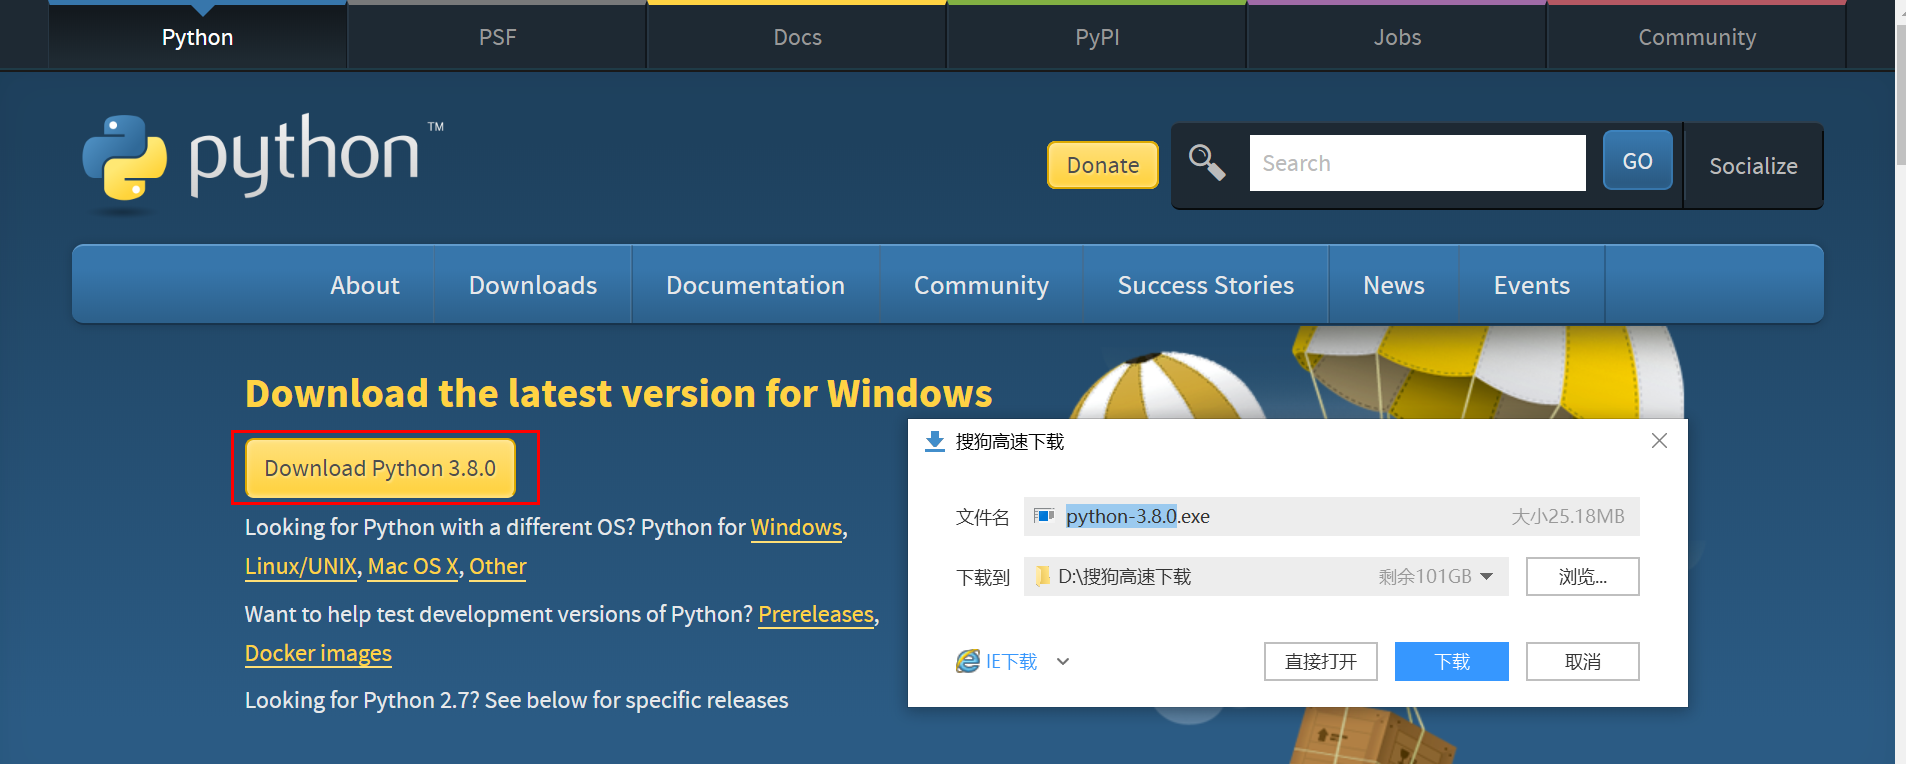
\includegraphics[height=1.3in, width=3.4in, viewport=0 0 1906 694,clip]{Figures/python_download-windows.png}
\label{Python-download_windows}
\end{figure}
\item 点击下载
            \end{itemize}
\end{frame}

\begin{frame}
	\frametitle{\textrm{Windows}系统安装\textrm{Python}}
        运行安装程序
            \begin{itemize}
                \item 双击下载的安装包,进入安装向导
		\item 推荐勾选\textrm{Add Python to PATH}选项\\
			{\fontsize{7.2pt}{4.2pt}\selectfont{方便后续在命令行中使用\textrm{Python}}}
		\item 选择\textrm{Customize installation}(自定义安装)\\
		{\fontsize{7.2pt}{4.2pt}\selectfont{勾选需要安装的组件,如\textcolor{magenta}{\textrm{pip}}~(\textrm{Python}包管理工具)等}}
		\item 点击\textrm{Install}开始安装
            \end{itemize}
\begin{figure}[h!]
%\vspace*{-0.15in}
\centering
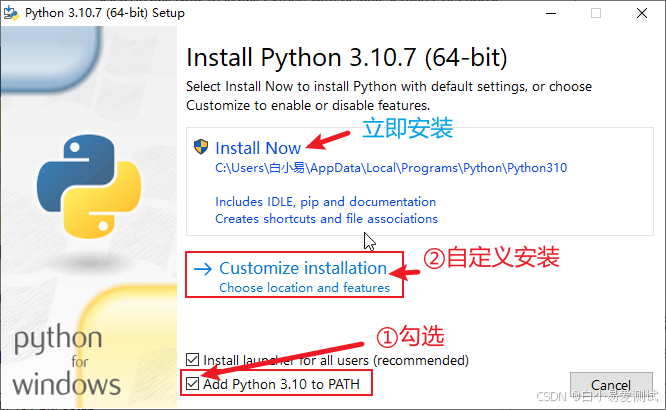
\includegraphics[height=0.8in, width=1.3in, viewport=0 0 666 410,clip]{Figures/python_install-windows-1.png}
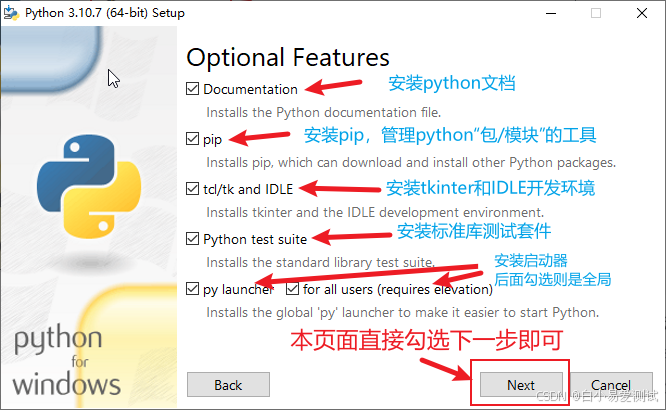
\includegraphics[height=0.8in, width=1.3in, viewport=0 0 666 410,clip]{Figures/python_install-windows-2.png}
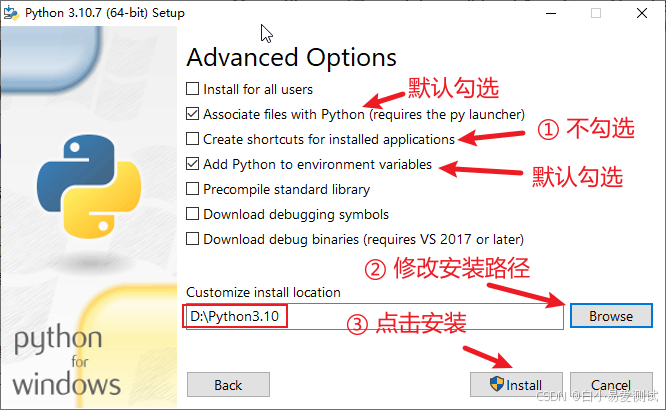
\includegraphics[height=0.8in, width=1.3in, viewport=0 0 666 410,clip]{Figures/python_install-windows-3.png}
%\caption{\tiny \textrm{Pseudopotential for metallic sodium, based on the empty core model and screened by the Thomas-Fermi dielectric function.}}%(与文献\cite{EPJB33-47_2003}图1对比)
\label{Python-install_windows}
\end{figure}
\end{frame}

\begin{frame}
	\frametitle{\textrm{Windows}系统配置\textrm{Python}}
\begin{figure}[h!]
\vspace*{-0.18in}
\centering
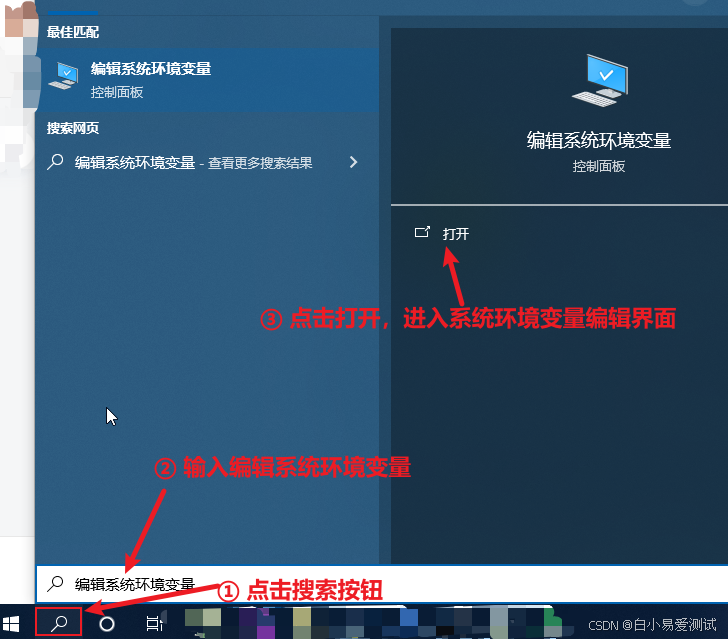
\includegraphics[height=1.3in, width=1.5in, viewport=0 0 728 639,clip]{Figures/python_config-windows-1.png}
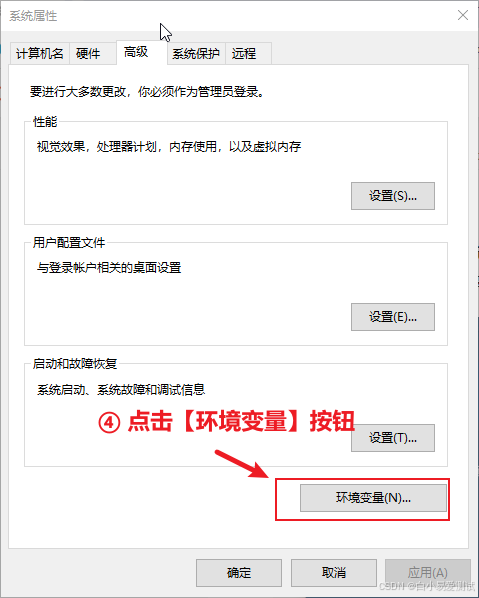
\includegraphics[height=1.3in, width=1.2in, viewport=0 0 479 598,clip]{Figures/python_config-windows-2.png}\\
\hspace*{-0.11in}
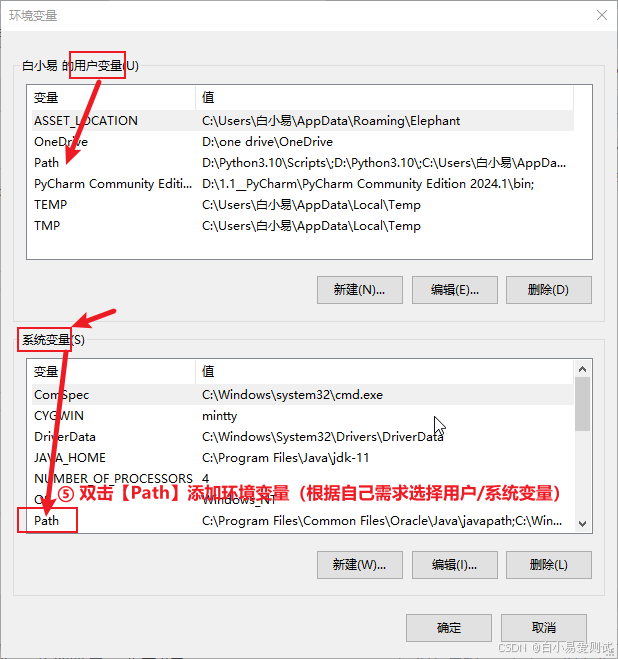
\includegraphics[height=1.4in, width=1.3in, viewport=0 0 618 659,clip]{Figures/python_config-windows-3.png}
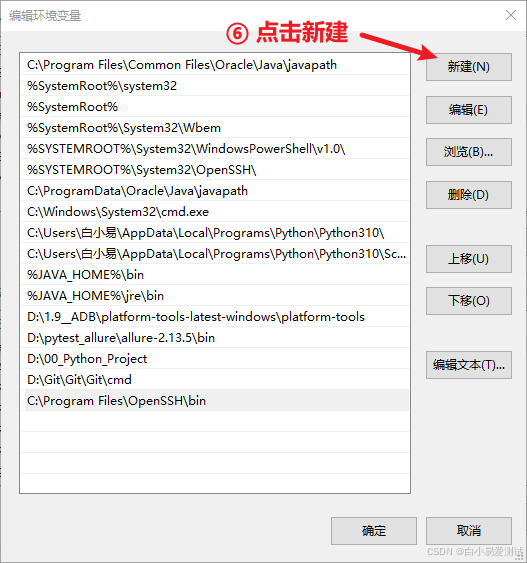
\includegraphics[height=1.4in, width=1.35in, viewport=0 0 527 563,clip]{Figures/python_config-windows-4.png}
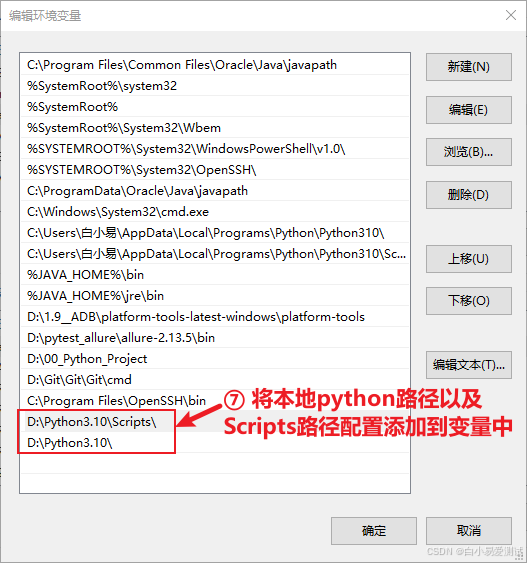
\includegraphics[height=1.4in, width=1.35in, viewport=0 0 527 563,clip]{Figures/python_config-windows-5.png}\\
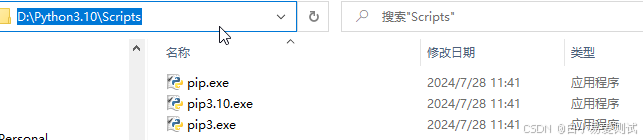
\includegraphics[height=0.35in, width=1.8in, viewport=0 0 640 140,clip]{Figures/python_config-windows-pip.png}
\label{Python-config_windows}
\end{figure}
\end{frame}

% 幻灯片5:Linux系统安装Python
\begin{frame}[fragile]
	\frametitle{\textrm{Linux}系统安装\textrm{Python}}
	    基于\textrm{Debian}或\textrm{Ubuntu}系统
            \begin{itemize}
		    \item 打开终端,运行命令 \verb|sudo apt-get update|\\
			    {\fontsize{7.2pt}{4.2pt}\selectfont{\textcolor{magenta}{\%更新软件源}}}
               \item 运行命令 \verb|sudo apt-get install python3|\\
		       {\fontsize{7.2pt}{4.2pt}\selectfont{\textcolor{magenta}{\%安装\textrm{Python~3}~(系统默认安装的可能是\textrm{Python~2},需注意区分)}}}
                \item 安装完成后,运行命令 \verb|python3 --version|\\
			{\fontsize{7.2pt}{4.2pt}\selectfont{\textcolor{magenta}{\%查看\textrm{Python}版本}}}
            \end{itemize}
	    基于\textrm{Red~Hat}或\textrm{CentOS}系统
            \begin{itemize}
                \item 打开终端,运行命令 \verb|sudo yum install python3|\\
			{\fontsize{7.2pt}{4.2pt}\selectfont{\textcolor{magenta}{\%安装\textrm{Python~3}}}}
                \item 同样安装完成后,运行命令 \verb|python3 --version|\\
			{\fontsize{7.2pt}{4.2pt}\selectfont{\textcolor{magenta}{\%查看\textrm{Python}版本}}}
            \end{itemize}
\end{frame}

% 幻灯片6:MacOS系统安装Python
\begin{frame}[fragile]
	\frametitle{\textrm{MacOS}系统安装\textrm{Python}}
    \begin{itemize}
	    \item 使用\textrm{Homebrew}安装~(推荐)
            \begin{itemize}
		    \item 若未安装\textrm{Homebrew},先运行命令~\\
%			    \begin{verbatim}
%			    \end{verbatim}\\
			{\fontsize{8.2pt}{4.2pt}\selectfont{\verb|/bin/bash -c "$(curl -fsSL https://raw.githubusercontent.com/Homebrew/install/HEAD/install.sh)"|}}
%			    \begin{verbatim}
%			    \end{verbatim}\\
			    {\fontsize{7.2pt}{4.2pt}\selectfont{\textcolor{magenta}{\%安装\textrm{Homebrew}}}}
                \item 安装完成后,运行命令 \verb|brew install python|\\
			{\fontsize{7.2pt}{4.2pt}\selectfont{\textcolor{magenta}{\%安装\textrm{Python}}}}
%                \item 安装过程中可能需要输入用户密码,输入后按回车键继续
            \end{itemize}
        \item 使用官方安装包安装
            \begin{itemize}
		    \item 访问\textrm{Python}官方网站下载适合\textrm{MacOS}的安装包
                \item 双击安装包,按安装向导提示,完成安装
            \end{itemize}
    \end{itemize}
                安装完成,运行命令 \verb|python3 --version|\\
			{\fontsize{7.2pt}{4.2pt}\selectfont{\textcolor{magenta}{\%查看\textrm{Python}版本}}}
\end{frame}

% 幻灯片7:安装后的验证与测试
\begin{frame}
	\frametitle{\textrm{Python}测试与运行:~以\textrm{Windows}系统为例}
\begin{figure}[h!]
\vspace*{-0.15in}
\centering
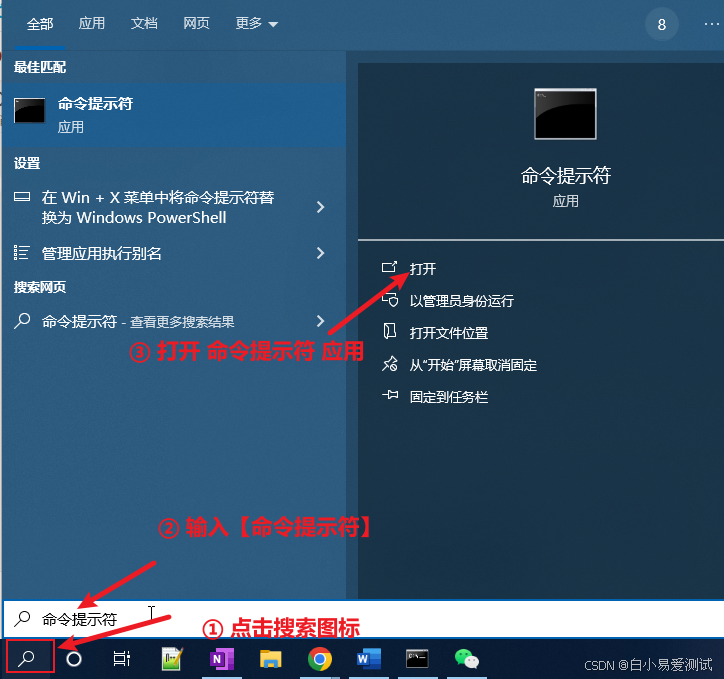
\includegraphics[height=1.3in, width=1.4in, viewport=0 0 724 627,clip]{Figures/python_config-windows-6.png}\\
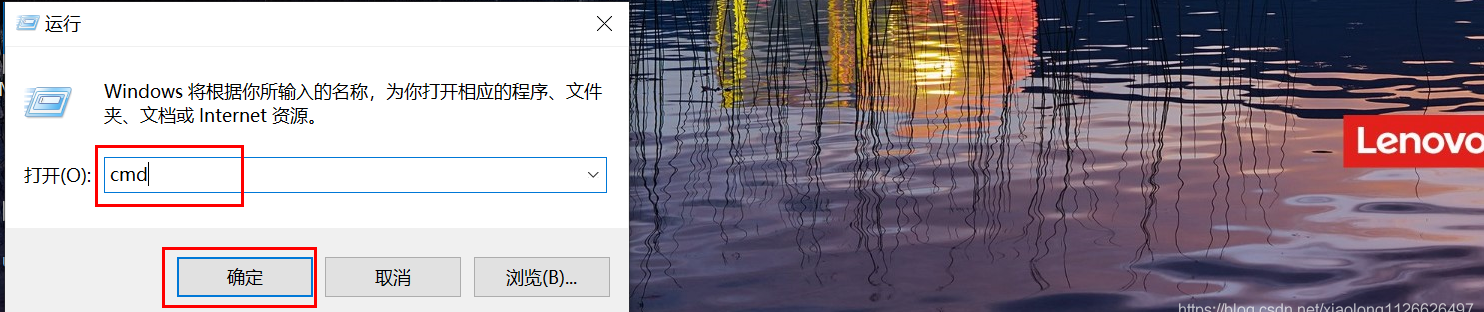
\includegraphics[height=0.6in, width=3.5in, viewport=0 0 1484 312,clip]{Figures/python_command-windows-1.png}
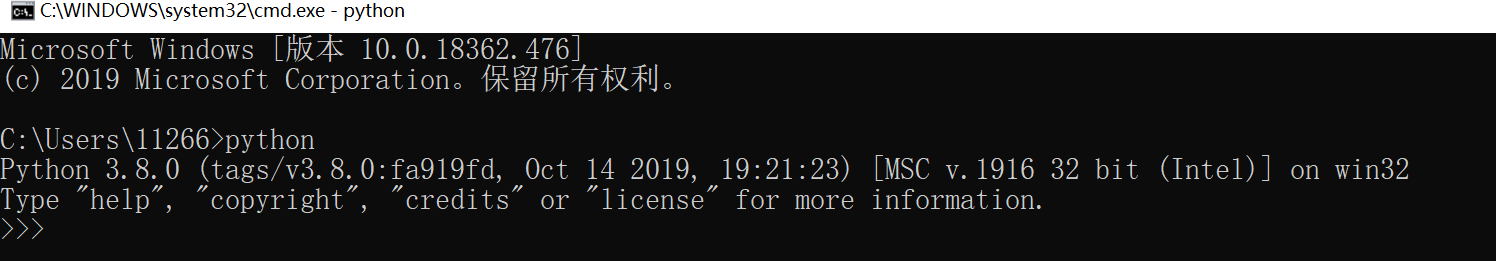
\includegraphics[height=0.5in, width=3.5in, viewport=0 0 1496 261,clip]{Figures/python_command-windows-2.png}
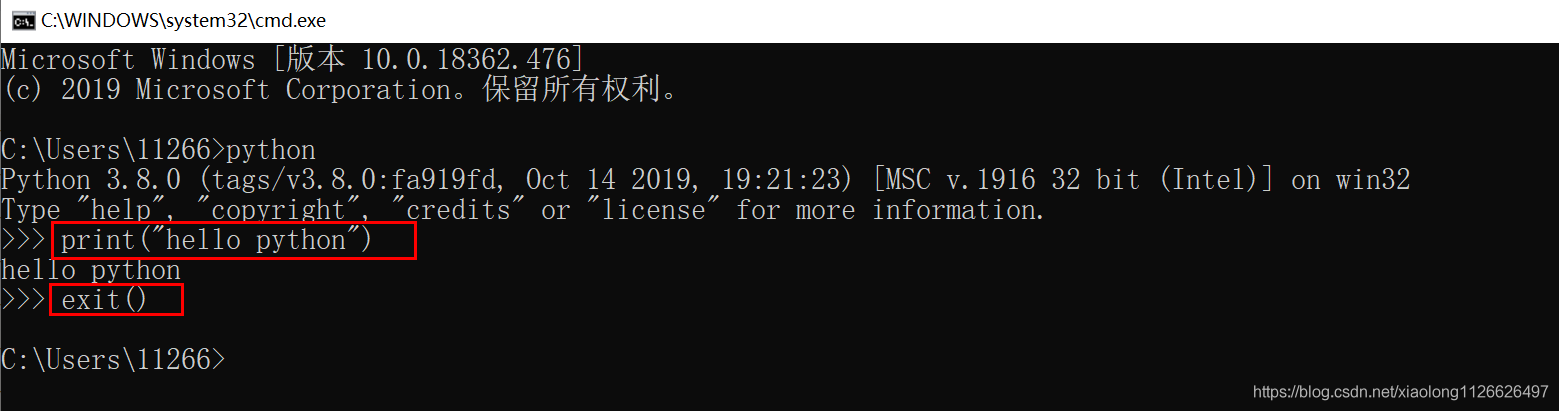
\includegraphics[height=0.6in, width=3.5in, viewport=0 0 1559 387,clip]{Figures/python_command-windows-3.png}
%\caption{\tiny \textrm{Pseudopotential for metallic sodium, based on the empty core model and screened by the Thomas-Fermi dielectric function.}}%(与文献\cite{EPJB33-47_2003}图1对比)
\label{Python-run_windows}
\end{figure}
\end{frame}

%\begin{frame}[fragile]
%    \frametitle{安装后的验证与测试}
%    \begin{itemize}
%        \item 验证Python是否安装成功
%            \begin{itemize}
%                \item 打开命令行(Windows下为CMD或PowerShell,Linux和MacOS下为终端)
%                \item 输入命令\verb|python --version|(若安装的是Python 3,也可输入\verb|python3 --version|),显示Python版本号则安装成功
%            \end{itemize}
%        \item 测试Python运行
%            \begin{itemize}
%                \item 在命令行中输入\verb|python|(或\verb|python3|)进入Python交互式环境
%                \item 输入代码\verb|print("Hello, Python!")|,按回车键,若输出\verb|Hello, Python!|,则说明Python运行正常
%            \end{itemize}
%    \end{itemize}
%\end{frame}

% 幻灯片8:常见问题与解决方法
%\begin{frame}[fragile]
%    \frametitle{常见问题与解决方法}
%    \begin{itemize}
%        \item 安装过程中报错
%            \begin{itemize}
%                \item 检查网络连接是否正常,重新下载安装包
%		\item 确认系统是否满足\textrm{Python}安装要求~(如操作系统版本、硬件配置等)
%                \item 查看安装日志,根据错误信息在网上搜索解决方案
%            \end{itemize}
%        \item \textrm{pip}安装包失败
%            \begin{itemize}
%		    \item 检查\textrm{pip}版本,可通过命令\verb|pip install --upgrade pip|升级\textrm{pip}
%		    \item 更换\textrm{pip}源,如使用国内镜像源~(如清华大学镜像源:~\href{https://pypi.tuna.tsinghua.edu.cn/simple}{https://pypi.tuna.tsinghua.edu.cn/simple}),在命令行中运行\verb|pip config set global.index-url https://pypi.tuna.tsinghua.edu.cn/simple|
%            \end{itemize}
%    \end{itemize}
%\end{frame}

% 幻灯片9:总结与下一步
%\begin{frame}
%    \frametitle{总结与下一步}
%    \begin{itemize}
%        \item 总结
%            \begin{itemize}
%                \item 回顾在\textrm{Windows}、\textrm{Linux}和\textrm{MacOS}系统上安装\textrm{Python}的步骤
%                \item 强调安装过程中的注意事项和常见问题解决方法
%            \end{itemize}
%        \item 下一步
%            \begin{itemize}
%                \item 学习\textrm{Python}基础语法,开始编写\textrm{Python}程序
%                \item 探索\textrm{Python}丰富的库和框架,如\textrm{NumPy}、\textrm{pandas}、\textrm{Django}等
%                \item 参加\textrm{Python}社区,与其他开发者交流学习
%            \end{itemize}
%    \end{itemize}
%\end{frame}
\begin{frame}
	\frametitle{\textrm{Python}开发环境}
    \begin{itemize}
	    \item 文本编辑器:~如~\textrm{Sublime Text}、\textrm{VS Code}等
	    \item 集成开发环境\textrm{(IDE)}:如~\textrm{PyCharm}、\textrm{Jupyter Notebook}等
    \end{itemize}
\begin{figure}[h!]
\vspace*{-0.10in}
\centering
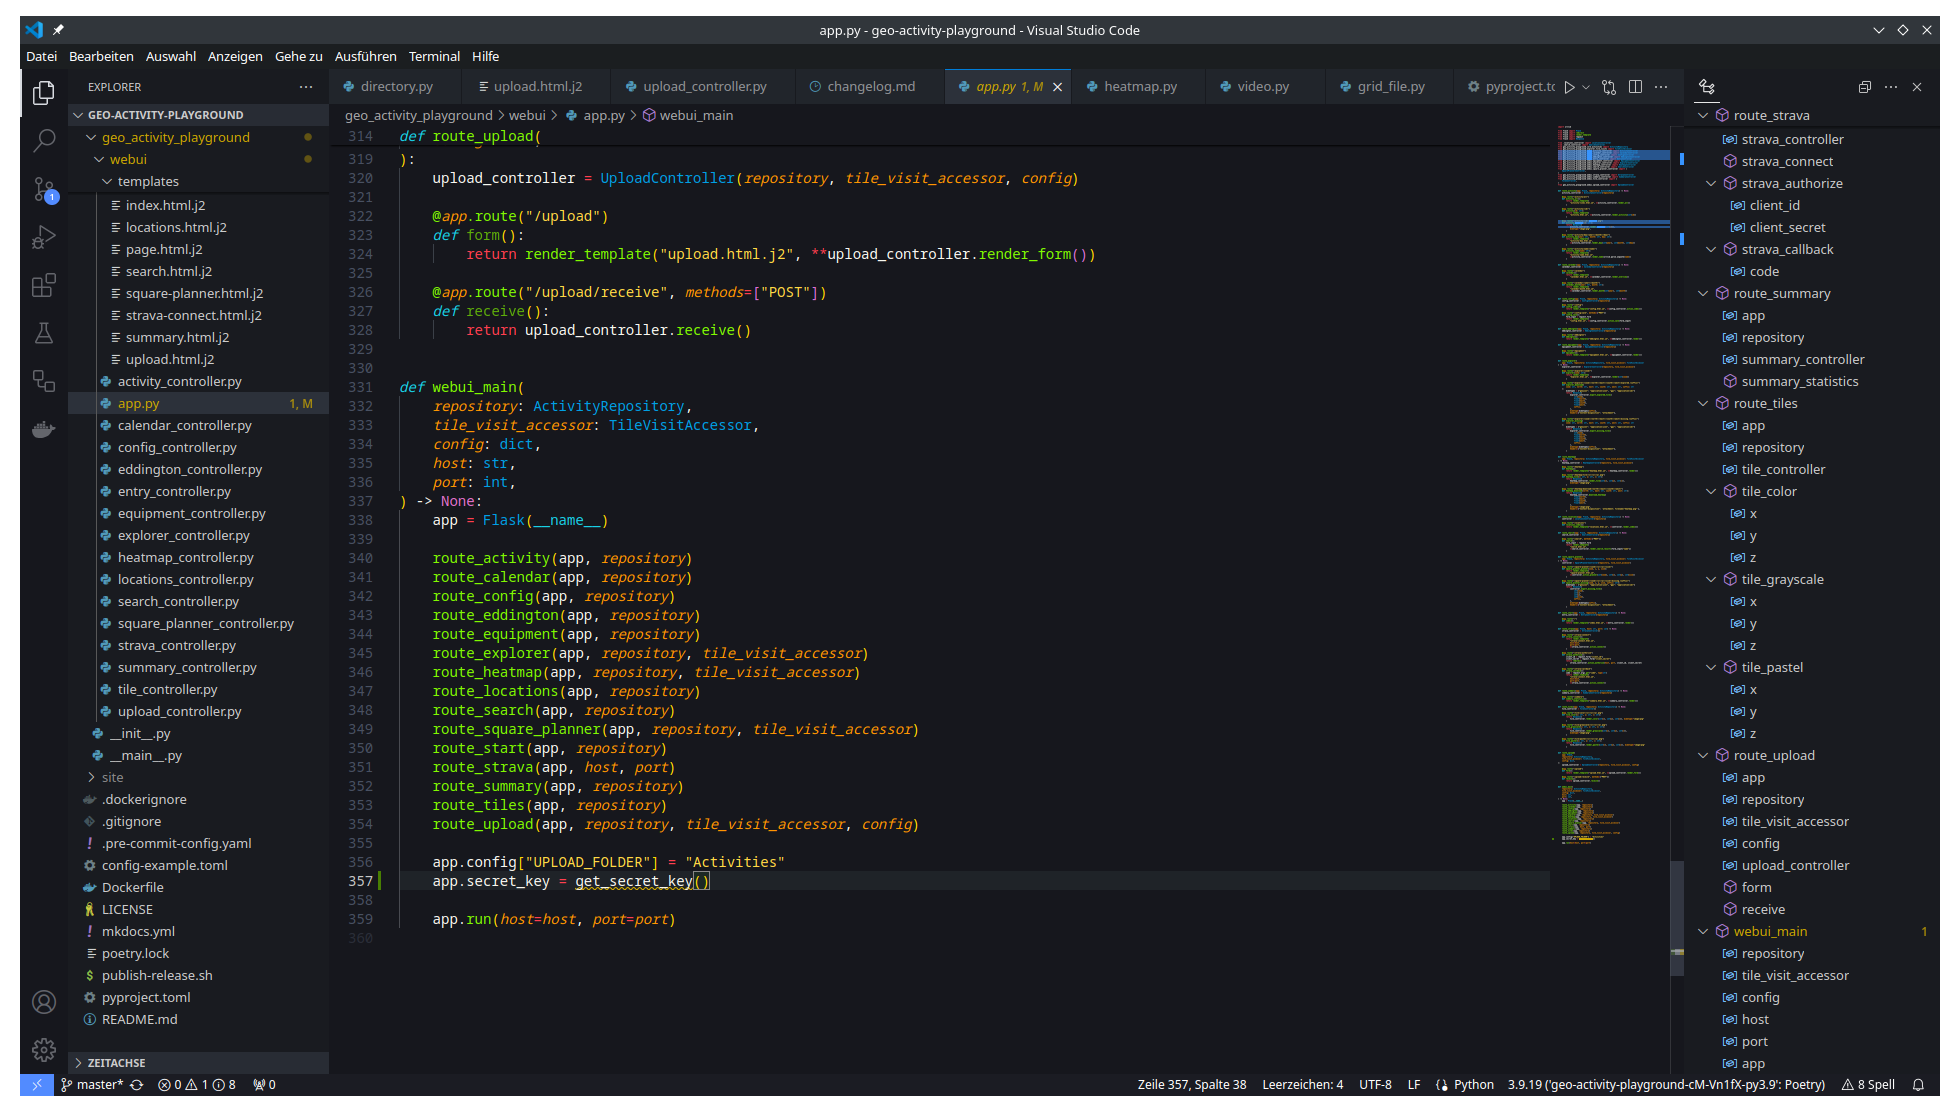
\includegraphics[height=1.3in, width=2.6in, viewport=0 0 1560 800,clip]{Figures/VS_code-python.png}
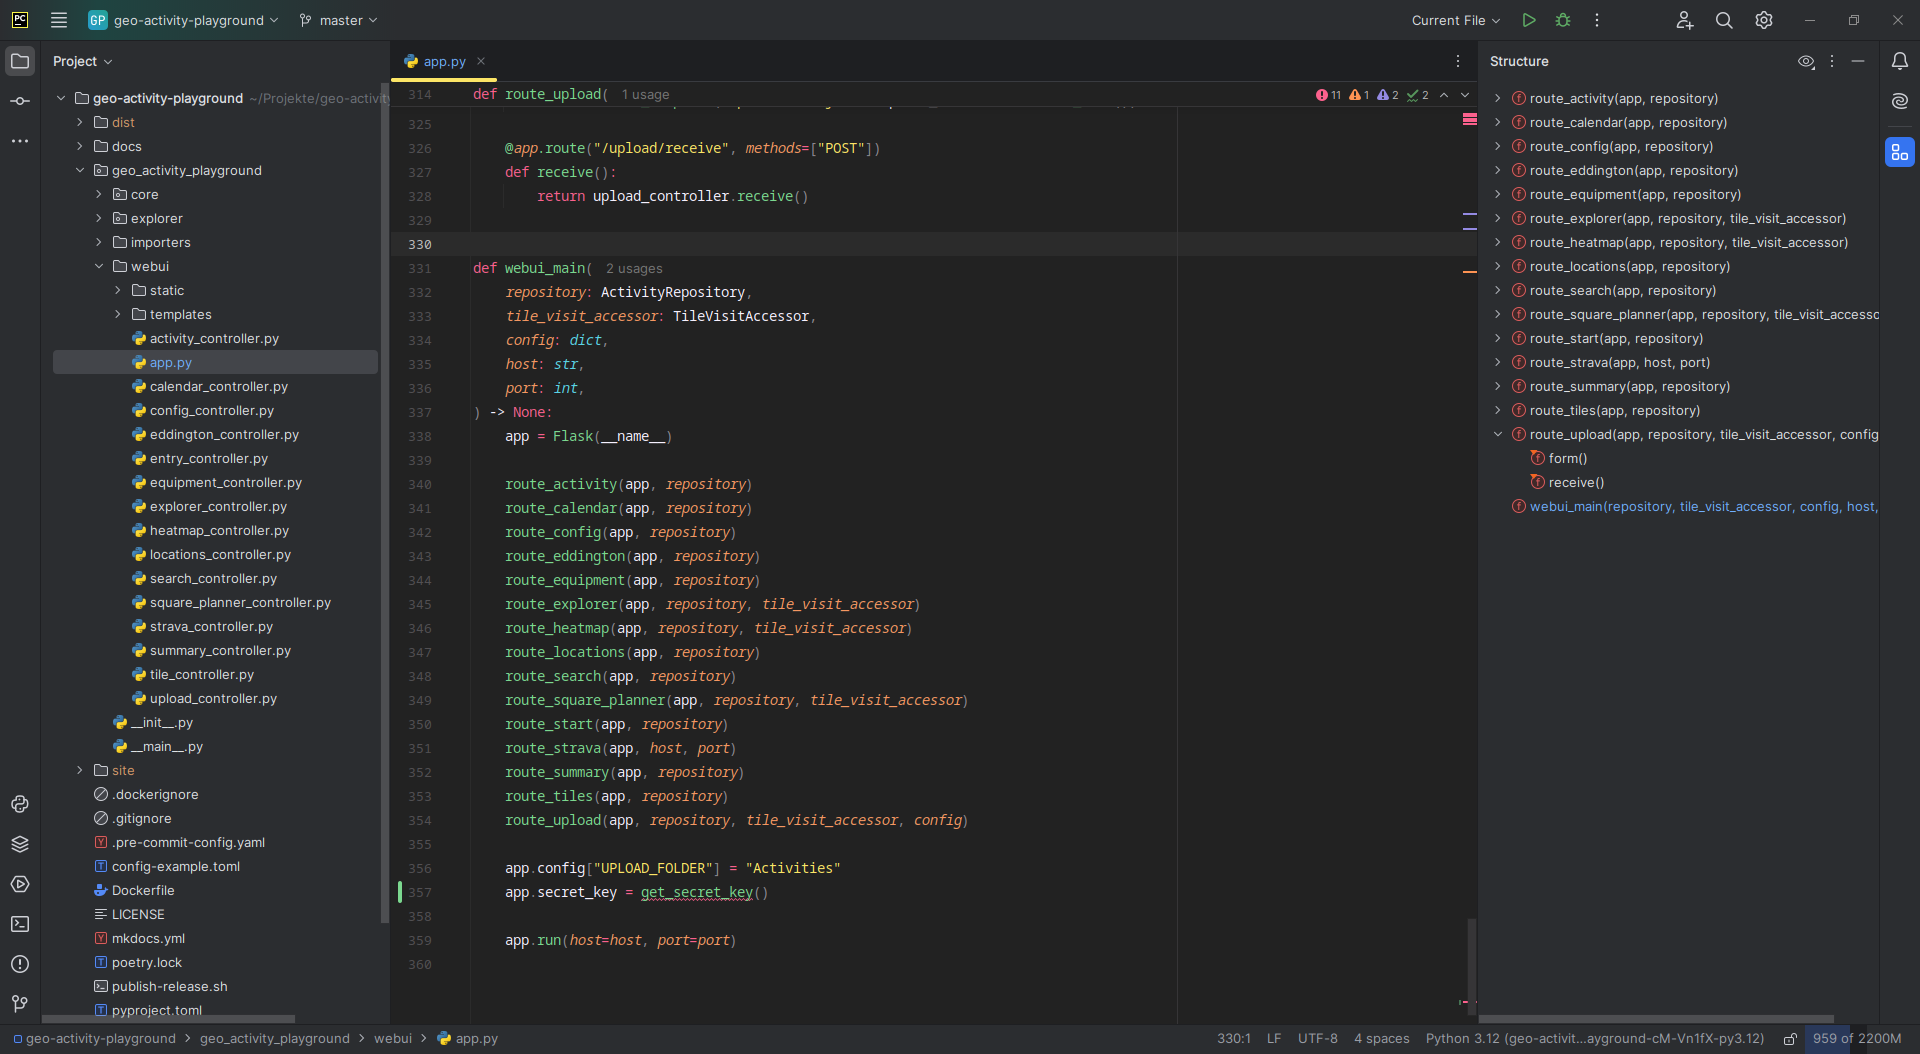
\includegraphics[height=1.3in, width=2.6in, viewport=0 0 1520 834,clip]{Figures/Pycharm-python.png}
%\caption{\tiny \textrm{Pseudopotential for metallic sodium, based on the empty core model and screened by the Thomas-Fermi dielectric function.}}%(与文献\cite{EPJB33-47_2003}图1对比)
\label{Python-editor}
\end{figure}
%    \begin{columns}
%        \column{0.5\textwidth}
%        \includegraphics[width=\textwidth]{vscode.png} % 替换为 VS Code 截图
%        \column{0.5\textwidth}
%        \includegraphics[width=\textwidth]{pycharm.png} % 替换为 PyCharm 截图
%    \end{columns}
\end{frame}

%% Jupyter Notebook 介绍
\section{\rm{Jupyter Notebook}使用介绍}
\begin{frame}
	\frametitle{\textrm{Jupyter Notebook}概述}
    \begin{itemize}
	    \item \textrm{Jupyter Notebook}是一个开源的\textrm{Web}应用程序,允许创建和共享包含代码、方程式、可视化和文本的文档
	    \item 支持多种编程语言,其中最常用的是\textrm{Python}
        \item 非常适合数据科学、机器学习等领域的快速原型开发和实验
    \end{itemize}
\begin{figure}[h!]
%\vspace*{-0.10in}
\centering
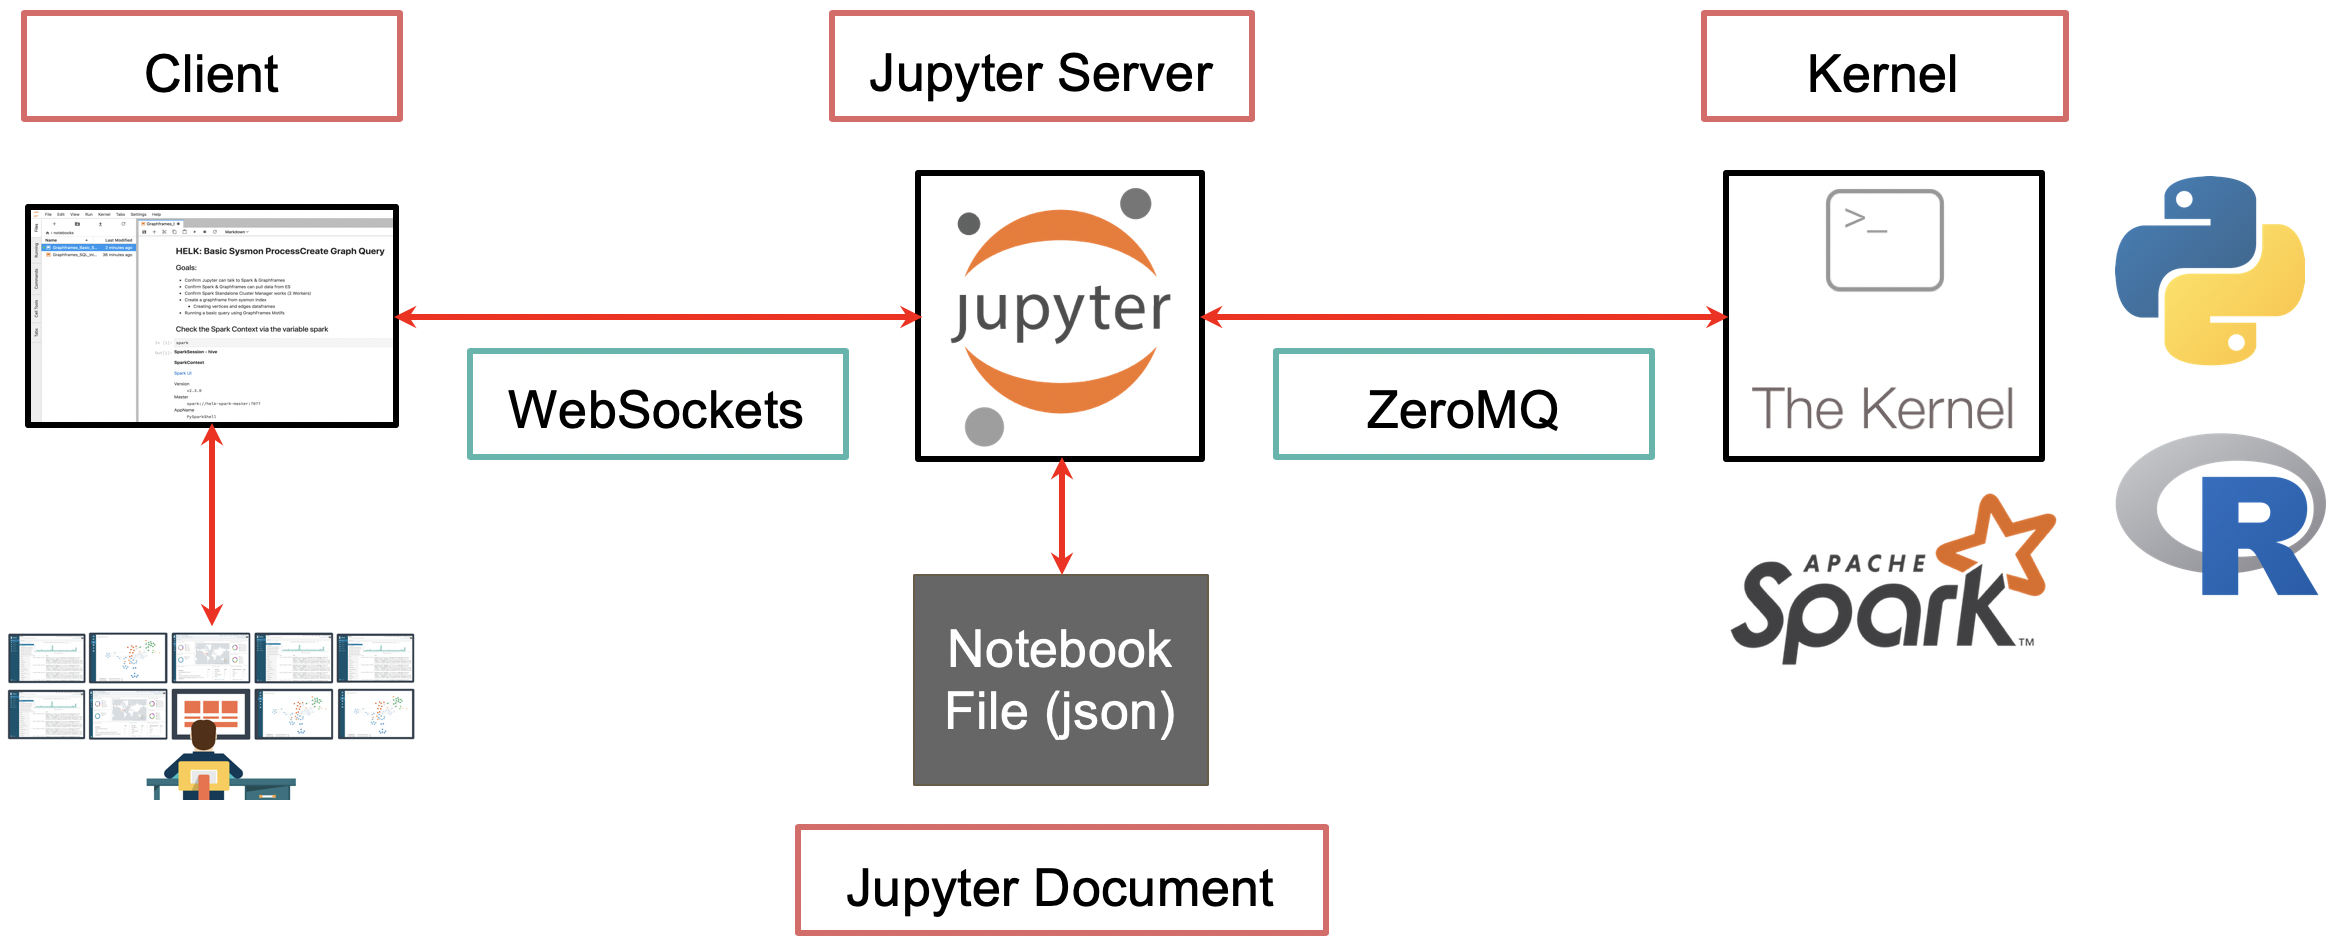
\includegraphics[height=1.6in, width=4.0in, viewport=0 0 1170 472,clip]{Figures/Jupyter_Architecture.png}
%\caption{\tiny \textrm{Pseudopotential for metallic sodium, based on the empty core model and screened by the Thomas-Fermi dielectric function.}}%(与文献\cite{EPJB33-47_2003}图1对比)
\label{Jupyter_notebook}
\end{figure}
%    \begin{center}
%        \includegraphics[width=0.6\textwidth]{jupyter_notebook.png} % 替换为 Jupyter Notebook 截图
%    \end{center}
\end{frame}
%
\begin{frame}[fragile]
	\frametitle{\textrm{Jupyter Notebook}的安装与启动}
	如果已经安装了\textrm{Python}和\textrm{pip},可用以下命令安装
    \begin{lstlisting}[style=pythonstyle]
pip install jupyter
    \end{lstlisting}
    安装完成后,在命令行中用命令启动
    \begin{lstlisting}[style=pythonstyle]
jupyter notebook
    \end{lstlisting}
    {\fontsize{7.2pt}{4.2pt}\selectfont{\textcolor{magenta}{\%将在默认浏览器中打开\textrm{Jupyter Notebook}界面}}}
\begin{figure}[h!]
\vspace*{-0.05in}
\centering
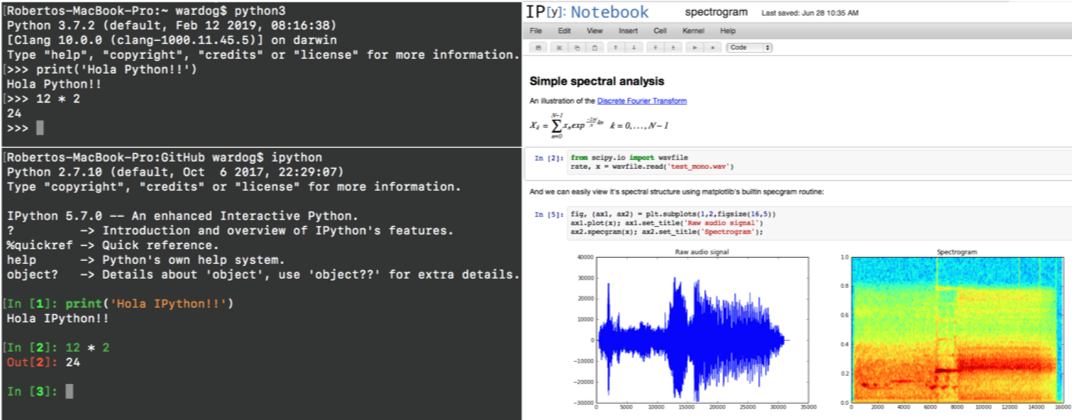
\includegraphics[height=1.6in, width=4.0in, viewport=0 0 520 220,clip]{Figures/Jupyter_ipython.png}
%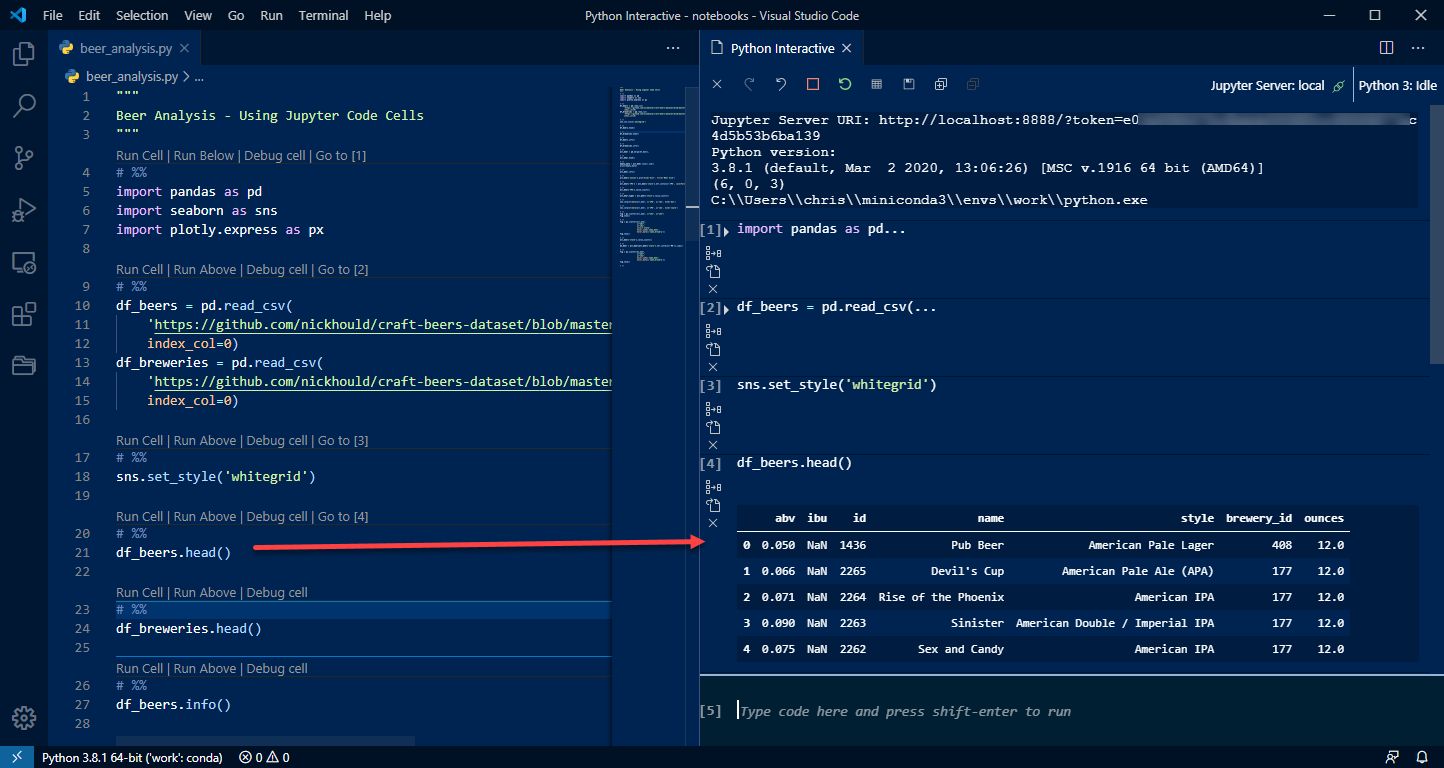
\includegraphics[height=1.6in, width=3.0in, viewport=0 0 1444 768,clip]{Figures/VS_code-vs-Jupyter_note.png}
%\caption{\tiny \textrm{Pseudopotential for metallic sodium, based on the empty core model and screened by the Thomas-Fermi dielectric function.}}%(与文献\cite{EPJB33-47_2003}图1对比)
\label{Jupyter_notebook_Framework}
\end{figure}
\end{frame}

\begin{frame}
	\frametitle{\textrm{Jupyter Notebook}基本格式}
%    \begin{itemize}
%	    \item 创建新的\textrm{Notebook}\\
%		    在\textrm{Jupyter Notebook}界面中,点击\textrm{``New''}按钮,选择\textrm{``Python~3''}创建新的\textrm{Python Notebook}
%        \item 单元格类型:~可以通过工具栏或快捷键切换单元格类型\\
		\textrm{Notebook}由多个单元格组成\\
		单元格类型有\textcolor{blue}{代码单元格}和\textcolor{blue}{\textrm{Markdown}单元格}
%        \item 运行单元格\\
%		在代码单元格中输入\textrm{Python}代码,按下\textrm{``Shift~+~Enter''}组合键运行代码
\begin{figure}[h!]
%\vspace*{-0.05in}
\centering
%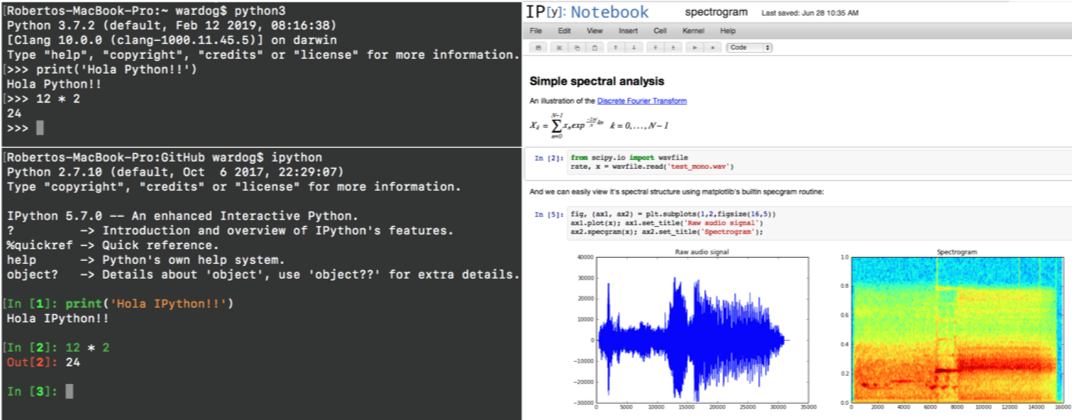
\includegraphics[height=1.6in, width=4.0in, viewport=0 0 520 220,clip]{Figures/Jupyter_ipython.png}
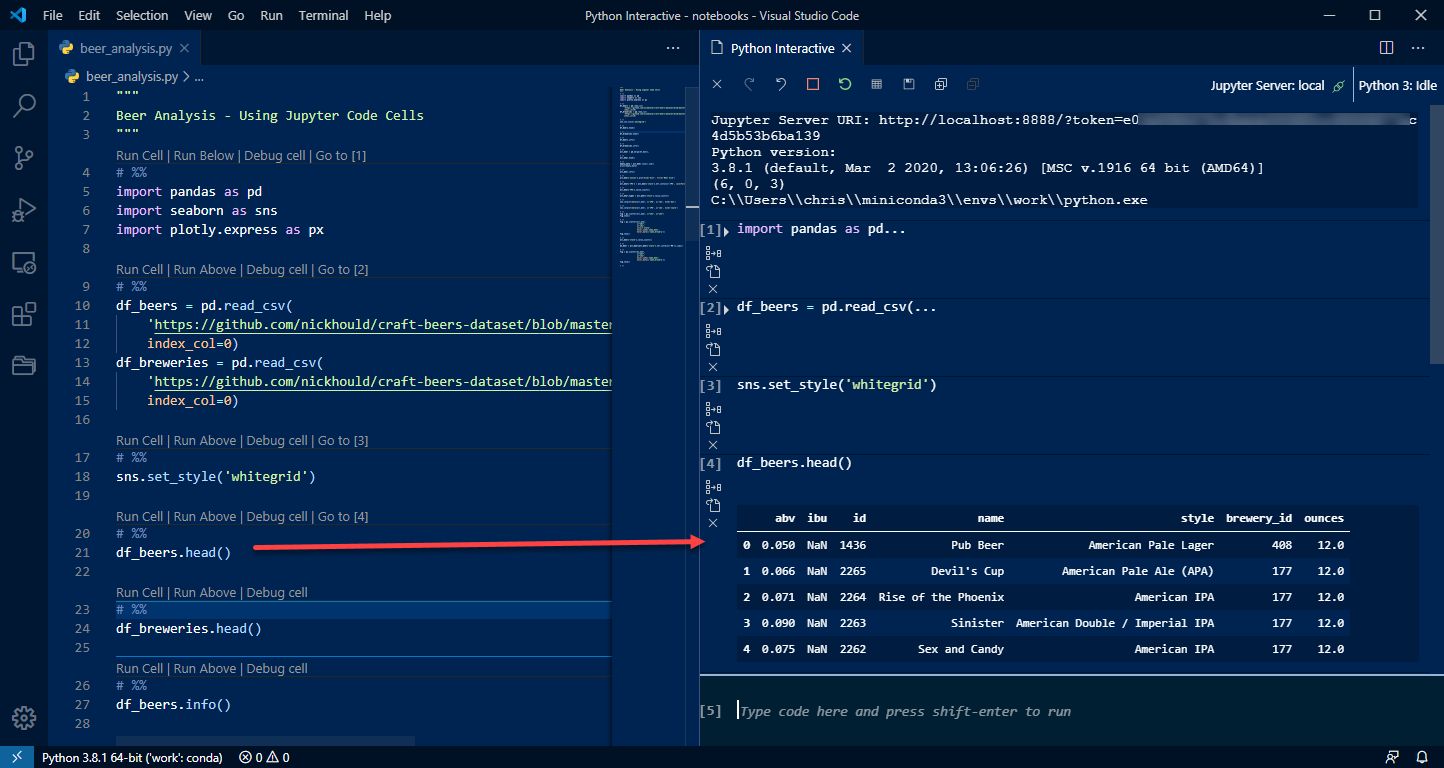
\includegraphics[height=2.0in, width=4.0in, viewport=0 0 1100 550,clip]{Figures/VS_code-vs-Jupyter_note.png}
%\caption{\tiny \textrm{Pseudopotential for metallic sodium, based on the empty core model and screened by the Thomas-Fermi dielectric function.}}%(与文献\cite{EPJB33-47_2003}图1对比)
\label{VS_code-vs-Jupyter_notebook}
\end{figure}
%	\item 保存\textrm{Notebook}\\
%		点击工具栏中的\textrm{``Save''}按钮或使用快捷键保存\textrm{Notebook}
%    \end{itemize}
\end{frame}

%% 基础语法
\section{基础语法}
\begin{frame}[fragile]
%	\frametitle{\textrm{Hello, World!}}
	\frametitle{\textrm{hello python}}
	\textrm{Python}的第一个程序
    \begin{lstlisting}[style=pythonstyle]
print("hello python")
    \end{lstlisting}
%print("Hello, World!")
%    解释:
    \begin{itemize}
	    \item \texttt{\textcolor{blue}{print}()} 是 \textrm{Python}的内置函数,用于输出内容到控制台
        \item 双引号内的内容是字符串
    \end{itemize}
\begin{figure}[h!]
%\vspace*{-0.15in}
\centering
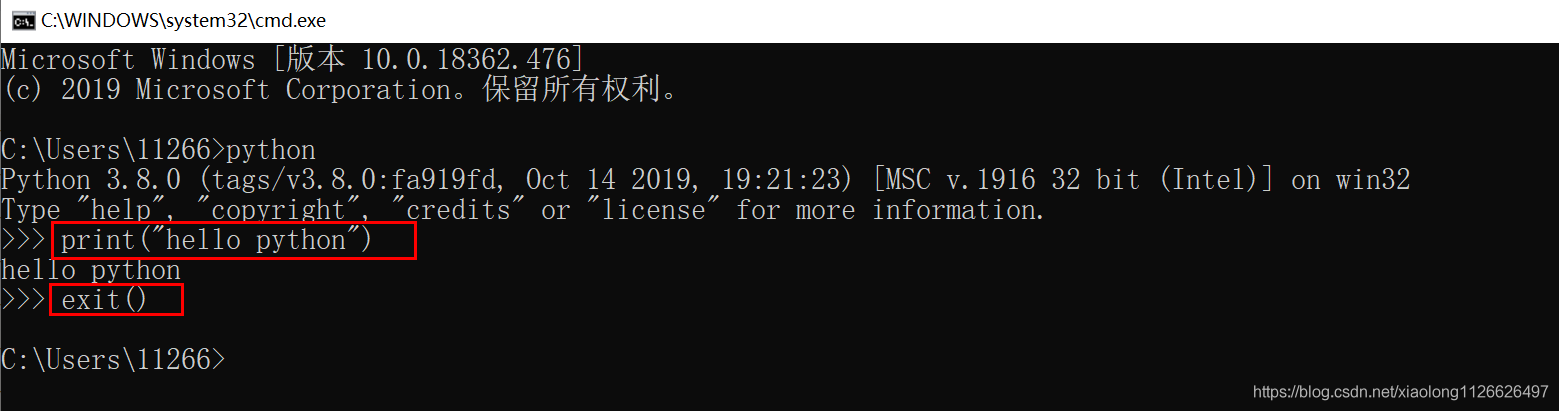
\includegraphics[height=0.9in, width=4.0in, viewport=0 0 1559 387,clip]{Figures/python_command-windows-3.png}
%\caption{\tiny \textrm{Pseudopotential for metallic sodium, based on the empty core model and screened by the Thomas-Fermi dielectric function.}}%(与文献\cite{EPJB33-47_2003}图1对比)
\label{Python-run_hello}
\end{figure}
\end{frame}
%
\begin{frame}[fragile]
	\frametitle{\textrm{Python}的变量与数据类型}
    \begin{itemize}
        \item 变量:~用于存储数据的容器
        \item 数据类型:
            \begin{itemize}
		    \item 整型\textrm{(int)}:~如\textrm{1, 2, -3}等
		    \item 浮点型\textrm{(float)}:~如\textrm{3.14, 2.718}等
		    \item 字符串\textrm{(str)}:~如\textrm{``Hello'', `World'}等
		    \item 布尔型\textrm{(bool)}:~\textrm{True}或\textrm{False}
            \end{itemize}
    \end{itemize}
    示例代码:
    \begin{lstlisting}[style=pythonstyle]
age = 20  # 整数
height = 1.75  # 浮点数
name = "Alice"  # 字符串
is_student = True  # 布尔值
    \end{lstlisting}
\end{frame}
%
\begin{frame}[fragile]
    \frametitle{输入与输出}
    输入:~\texttt{\textcolor{blue}{input}()}函数:~\textcolor{purple}{获取用户输入}
    \begin{lstlisting}[style=pythonstyle]
name = input("请输入拟的名字:")
print("你好," + name + "!")
    \end{lstlisting}
\begin{figure}[h!]
%\vspace*{-0.15in}
\centering
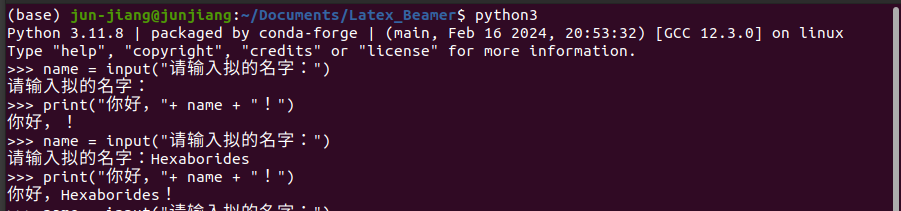
\includegraphics[height=0.9in, width=4.0in, viewport=0 9 901 211,clip]{Figures/python_Input-output.png}
%\caption{\tiny \textrm{Pseudopotential for metallic sodium, based on the empty core model and screened by the Thomas-Fermi dielectric function.}}%(与文献\cite{EPJB33-47_2003}图1对比)
\label{Python-Input_Output}
\end{figure}
%    解释:
\vspace*{-0.15in}
    \begin{itemize}
	    \item \texttt{\textcolor{blue}{input}()} 函数会暂停程序,等待用户输入内容,并将输入的内容作为字符串返回
	    \item 字符串可以使用 \texttt{+} 号拼接
    \end{itemize}
\end{frame}
%
%% 控制结构
\section{控制结构}
\begin{frame}[fragile]
    \frametitle{条件语句}
    条件语句用于根据条件执行不同的代码块。
    \begin{lstlisting}[style=pythonstyle]
age = 18
if age >= 18:
    print("你已经成年了!")
else:
    print("你还未成年。")
    \end{lstlisting}
%    解释:
    \begin{itemize}
	    \item \texttt{if} 语句后面跟着一个条件表达式\\
		    {\fontsize{8.2pt}{4.2pt}\selectfont{\textcolor{magenta}{如果条件为\textrm{True},则执行缩进的代码块}}}
	    \item \texttt{else} 语句后面的表达式\\
		    {\fontsize{8.2pt}{4.2pt}\selectfont{\textcolor{magenta}{用于处理条件为\textrm{False}的情况}}}
    \end{itemize}
\end{frame}

\begin{frame}[fragile]
    \frametitle{循环语句}
    循环语句用于重复执行一段代码
    \begin{itemize}
	    \item \texttt{\textcolor{blue}{for}} 循环:~用于遍历序列(如列表、字符串等)
        \begin{lstlisting}[style=pythonstyle]
fruits = ["apple", "banana", "cherry"]
for fruit in fruits:
    print(fruit)
        \end{lstlisting}
\item \texttt{\textcolor{blue}{while}} 循环:~根据条件重复执行代码块
        \begin{lstlisting}[style=pythonstyle]
count = 0
while count < 5:
    print(count)
    count = count + 1
        \end{lstlisting}
    \end{itemize}
\end{frame}
%
%% 函数
\section{自定义函数}
\begin{frame}[fragile]
    \frametitle{函数定义与调用}
\textcolor{purple}{函数}:~一段可重复使用的代码块
\begin{itemize}
	\item 自定义函数:~
    \begin{lstlisting}[style=pythonstyle]
def add(a, b):
    return a + b
    \end{lstlisting}
    \item 调用函数:~
    \begin{lstlisting}[style=pythonstyle]
result = add(3, 5)
print(result)
    \end{lstlisting}
\end{itemize}
%    解释:
    \begin{itemize}
	    \item 关键词~\texttt{\textcolor{blue}{def}}用于定义函数
	    \item 函数可以有参数{\fontsize{7.2pt}{4.2pt}\selectfont{\textrm{(如\texttt{a}和\texttt{b})}}}和返回值{\fontsize{7.2pt}{4.2pt}\selectfont{\textrm{(由关键词\texttt{\textcolor{blue}{return}}指定)}}}
    \end{itemize}
\end{frame}
%
%% 类与对象
\section{类与对象}
\begin{frame}[fragile]
    \frametitle{类的定义}
    \textcolor{purple}{类}:~对象的符号表示形式,定义了对象的属性和方法
    \begin{lstlisting}[style=pythonstyle]
class Person:
    def __init__(self, name, age):
        self.name = name
        self.age = age

    def introduce(self):
        print("我叫 {self.name},今年 {self.age} 岁。")

p = Person("Bob", 25)
p.introduce()
    \end{lstlisting}
%    解释:
    \begin{itemize}
	    \item \texttt{\textcolor{blue}{class}} 关键字用于定义类
        \item \texttt{\_\_init\_\_()} 是构造方法,用于初始化对象的属性
        \item \texttt{self} 代表类的实例
    \end{itemize}
\end{frame}
%
\begin{frame}[fragile]
    \frametitle{类的继承}
    继承允许一个类继承另一个类的属性和方法。
    \begin{lstlisting}[style=pythonstyle]
class Student(Person):
    def __init__(self, name, age, grade):
        super().__init__(name, age)
        self.grade = grade

    def study(self):
        print("{self.name} 正在学习,成绩是 {self.grade}。")

s = Student("Alice", 20, "A")
s.introduce()
s.study()
    \end{lstlisting}
%    解释:
    \begin{itemize}
        \item \texttt{Student} 类继承自 \texttt{Person} 类。
        \item \texttt{super()} 函数用于调用父类的方法。
    \end{itemize}
\end{frame}
%
%% 装饰器
\section{装饰器}
\begin{frame}[fragile]
    \frametitle{装饰器的概念}
    装饰器是一种特殊的函数,用于修改其他函数的行为。
    \begin{lstlisting}[style=pythonstyle]
def my_decorator(func):
    def wrapper():
        print("在函数执行前做一些事情")
        func()
        print("在函数执行后做一些事情")
    return wrapper

@my_decorator
def say_hello():
    print("Hello!")

say_hello()
    \end{lstlisting}
%    解释:
    \begin{itemize}
        \item \texttt{my\_decorator} 是一个装饰器函数,它接受一个函数作为参数,并返回一个新的函数。
        \item \texttt{@my\_decorator} 语法糖用于将 \texttt{say\_hello} 函数传递给 \texttt{my\_decorator} 装饰器。
    \end{itemize}
\end{frame}
%
%% 模块与包
\section{模块与包}
\begin{frame}[fragile]
    \frametitle{模块}
    模块是一个包含 Python 代码的文件。
    导入模块:
    \begin{lstlisting}[style=pythonstyle]
import math
result = math.sqrt(16)
print(result)
    \end{lstlisting}
%    解释:
    \begin{itemize}
        \item \texttt{import} 关键字用于导入模块。
        \item 可以使用模块中的函数和变量。
    \end{itemize}
\end{frame}
%
\begin{frame}[fragile]
    \frametitle{包}
    包是一个包含多个模块的目录。
    导入包中的模块:
    \begin{lstlisting}[style=pythonstyle]
import mypackage.mymodule
mypackage.mymodule.my_function()
    \end{lstlisting}
    或者使用 \texttt{from...import} 语句:
    \begin{lstlisting}[style=pythonstyle]
from mypackage.mymodule import my_function
my_function()
    \end{lstlisting}
\end{frame}
%
%% 总结
\section{总结}
\begin{frame}
    \frametitle{总结}
    \begin{itemize}
        \item 了解了 Python 的基本概念和安装方法。
        \item 学习了 Python 的基础语法,包括变量、数据类型、输入输出等。
        \item 掌握了控制结构(条件语句、循环语句)和函数的使用。
        \item 学习了类与对象、继承和装饰器的知识。
        \item 了解了 Jupyter Notebook 等开发环境的使用。
        \item 了解了模块和包的概念及使用方法。
    \end{itemize}
    继续学习,探索更多 Python 的知识!
\end{frame}
%
